\documentclass{article} 
\usepackage{amsmath,amsthm}     
\usepackage{graphicx}     
\usepackage{hyperref} 
\usepackage{url}
\usepackage{amsfonts} 
\usepackage{multicol}
\usepackage{tikz}
\usepackage{smartdiagram}
\usepackage{tabularx}
\usepackage{enumitem}
\usepackage{hyperref}
\usepackage[ruled,vlined]{algorithm2e}

\DeclareMathOperator{\diag}{diag}
\DeclareMathOperator{\E}{\mathbb{E}}
\usetikzlibrary{positioning,chains,fit,shapes,calc}
\theoremstyle{theorem}
\newtheorem{theorem}{Theorem}

\theoremstyle{definition}
\newtheorem*{definition}{Definition}
\newtheorem{assumption}{Assumption}
\newtheorem*{remark}{Remark}
\newtheorem{proposition}{Proposition}

\allowdisplaybreaks
\usepackage{collectbox}
\makeatletter
\newcommand{\mybox}{%
	\collectbox{%
		\setlength{\fboxsep}{1pt}%
		\fbox{\BOXCONTENT}%
	}%
}
\@addtoreset{footnote}{page}
\makeatother

%%%%%%%%%%%%%%%%%%%%%%%%%%%%%%%%%%%%%%%%%%%%%%%%%%
\begin{document}

	\newpage
	\title{Pruning in federated learning}
	
	\author{Hoang Trung Hieu
		%\scriptsize \\    
	%Eötvös Loránd University \\               
		%hthtb22@gmail.com
	}                      
	\date{2020}
	\maketitle
	
	\noindent
	\begin{abstract}		
	\end{abstract}

	\section{Neural network pruning}
	To reduce the size of network there a quite a few techniques were introduced by removing parameters. In $\cite{cite1}$, they used the second-order Taylor expansion, but computing in Hessian matrix is unattainable to modern deep neural network. It shows that a fully trained dense network can be pruned to little parameters without degrading performance too much. In case of training a sparse sub-network, the lottery ticket hypothesis was introduced in  \cite{cite3}, \cite{cite4}. They believe that dense networks contain sparse sub-networks that can be trained to perform as good as the original dense model.\\
	In gereral, in order to develop any competitive pruning technique, it requires to answer the following 4 questions:
	\begin{itemize}
		\item \textbf{What connectivity structures to prune?}
		\textit{ Unstructured pruning} does not consider any relationships between the pruned weights. \textit{Structured pruning}, on the other hand, prunes weights in groups. \textit{Local pruning} enforces that one prunes $p
		 $ percent of weights from each layer. \textit{Global pruning}, on the other hand, is unrestricted and simply requires that the total number of weights across the entire network is pruned by $p$ percent.
		\item \textbf{What is the pruning criterion?} A popular technique is magnitude-based pruning (\cite{cite2}) that keep the large magnitude weights since it has more impact on the function fit and should be pruned less. In addition to this, there are technique which use gradient-based methods or even higher-order curvature information.
		\item \textbf{When we prune?} There are 3 stamps when can apply pruning: before (initialisation-based) , during (training-based) and after training.  \textit{Pruning before training} performs the opting based on the untrained weights. \textit{Pruning during training}, on the other hand, is often associated with regularization and ideas of dropout. When \textit{pruning after the training} has converged the performance often decreases, which makes it necessary to retrain/fine-tune and to give the network a chance to readjust. 
		\item \textbf{How often to perform the pruning step?} \textit{Iterative} procedures prune only a small number of weights after one training run but reiterate the train - score - prune - rewind cycle. On the other hand, \textit{one-shot pruning} (\cite{cite6}) performs only a single time at the end of training.
	\end{itemize}
 
\begin{center}
	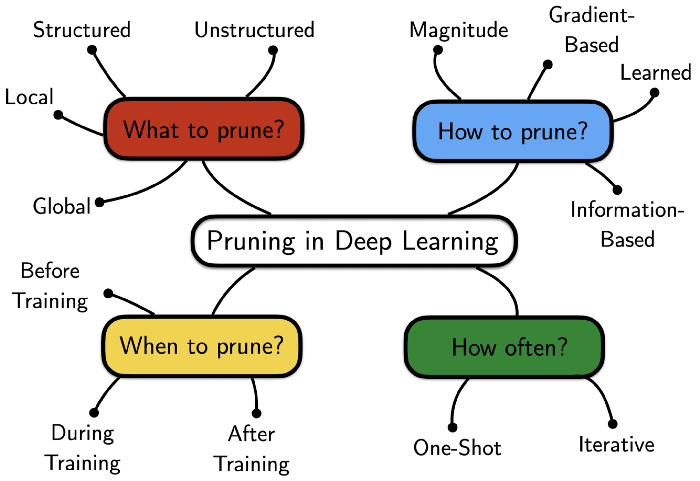
\includegraphics[scale=0.3]{overall}\\
	\figurename[1]{ What, When, How and How often to prune?}
\end{center}
In \cite{cite3}, they propose iterative magnitude pruning, in particular, unstructed, magnitude-based, iterative and initialisation-based prunning. In\cite{cite5}, they suggested the mixed-method which combines two factor magnitude and gradient sensitivity into one criterion by taking the multiplication.
\section{Federated Learning pruning}
	\begin{thebibliography}{5}
	\bibitem{cite1}
	Yann LeCun, John S Denker, and Sara A Solla. \textit{Optimal brain damage}. In Advances in neural information processing systems, pages 598–605, 1990.
	\bibitem{cite2}
 Song Han, Jeff Pool, John Tran, and William Dally.\textit{ Learning both weights and connections for
efficient neural network.} In Advances in neural information processing systems, pages 1135–1143,
2015.
\bibitem{cite3}
Jonathan Frankle and Michael Carbin.\textit{ The lottery ticket hypothesis: Finding sparse, trainable
neural networks.} In ICLR, 2019
\bibitem{cite4}
Ari Morcos, Haonan Yu, Michela Paganini, and Yuandong Tian.\textit{ One ticket to win them all: generalizing lottery ticket initializations across datasets and optimizers.} In Advances in Neural Information Processing Systems, pages 4933–4943, 2019.
\bibitem{cite5}
Dániel Lévai, Zsolt Zombori. \textit{Data-dependent Pruning to find the Winning Lottery Ticket}, \href{https://arxiv.org/abs/2006.14350}{https://arxiv.org/abs/2006.14350}, 2020
\bibitem{cite6}
Namhoon Lee, Thalaiyasingam Ajanthan, and Philip Torr. Snip: \textit{Single-shot network pruning
based on connection sensitivity.} In International Conference on Learning Representations, 2019.
\href{https://openreview.net/forum?id=B1VZqjAcYX}{https://openreview.net/forum?id=B1VZqjAcYX} .
\end{thebibliography}

\end{document}